\documentclass[pdftex, xcolor=pdftex, dvipsnames, handout]{beamer}

\usetheme{MA211}
\usepackage{thumbpdf}
\usepackage{wasysym}
%\usepackage{ucs}
\usepackage[utf8]{inputenc}
\usepackage{pgf,pgfarrows,pgfnodes,pgfautomata,pgfheaps,pgfshade}
\usepackage{verbatim}

\usepackage{eurosym}

\DeclareMathOperator*{\median}{median}
\usepackage{calc}               % Simple computations with LaTeX variables
%\usepackage[hang]{caption2}     % Improved captions

\usepackage{graphicx}           % Standard graphics package

\usepackage{amsmath, amsthm, amssymb}


\newcommand{\fquad}{\mbox{\qquad}}
\newcommand{\bull}{$\bullet$ }

\newcommand {\I} {\mathcal I}
\newcommand {\calI} {\mathcal I}
\def\disint{\displaystyle\int}

\DeclareMathOperator{\D}{d}
\newcommand{\dydx}{\frac{\D y}{\D x}}

%\definecolor{gray}{rgb}{0.69, 0.69, 0.69} \newcommand{\gray}[1]{\textcolor{gray}{#1}}
\definecolor{dogreen}{rgb}{0.33, 0.42, 0.18} \newcommand{\dogreen}[1]{\textcolor{dogreen}{#1}}
\definecolor{maroon}{rgb}{.5,0.2,0.2}\newcommand{\maroon}[1]{\textcolor{maroon}{#1}}
\definecolor{greena}{rgb}{.1,0.581,0.1}\newcommand{\greena}[1]{\textcolor{greena}{#1}}

\definecolor{blue4}{rgb}{0,0,.545}
\newcommand{\Blue}[1]{\textcolor{blue}{#1}}
\newcommand{\Red}[1]{\textcolor{red}{#1}}
\definecolor{pink}{rgb}{1.,0.75,0.8}
\definecolor{darkred}{rgb}{0.5,0.0,0.0}
\definecolor{darkgreen}{rgb}{0,0.3,0.3}
\definecolor{purple}{rgb}{0,0.3,0.3}
\definecolor{darkblue}{rgb}{0.0, 0.0, .5}
\definecolor{dpurple}{rgb}{.3,.0,.3}
\newcommand{\Green}[1]{\textcolor{darkgreen}{#1}}
\newcommand{\DRed}[1]{\textcolor{darkred}{#1}}
\newcommand{\DBlue}[1]{\textcolor{darkblue}{#1}}
\newcommand{\Purple}[1]{\textcolor{dpurple}{#1}}
\newcommand{\Emph}[1]{\textcolor{darkred}{\textbf{\it #1}}}
\newcommand{\remph}[1]{\textcolor{darkred}{\textbf{\emph{#1}}}}
\newcommand{\bemph}[1]{\textcolor{darkblue}{\textbf{\emph{#1}}}}
\newcommand{\gemph}[1]{\textcolor{darkgreen}{\textbf{\emph{#1}}}}
\newcommand{\Bf}[1]{\textcolor{darkblue}{\textbf{#1}}}
\newcommand{\Gf}[1]{\textcolor{darkgreen}{\textbf{#1}}}
\newcommand{\Rf}[1]{\textcolor{red}{\textbf{#1}}}
\newcommand{\Rmf}[1]{\textcolor{red}{\mathbf{#1}}}

\newcommand{\Conj}[1]{\overline{#1}}

\newcommand{\code}[1]{\textcolor{darkblue}{\texttt{\textbf{#1}}}}
\newcommand{\icode}[1]{{\blue\texttt{\textbf{\emph{#1}}}}}
\newcommand{\gcode}[1]{{\Green{\texttt{\textbf{\emph{#1}}}}}}
\newcommand{\out}[1]{\texttt{\emph{\textbf{\Green{#1}}}}}





\newenvironment{vminipage}%
{\begin{Sbox}\begin{minipage}\begin{small}\begin{verbatim}}%
{\end{verbatim}\end{small}\end{minipage}\end{Sbox}\fbox{\TheSbox}}

\newenvironment{nminipage}%
{\begin{Sbox}\begin{minipage}}%
{\end{minipage}\end{Sbox}\fbox{\TheSbox}}


\let\Arg\relax\DeclareMathOperator{\Arg}{\mathtt{Arg}}
\let\Arg\relax\DeclareMathOperator{\e}{\mathtt{e}}

\newcommand {\AND} {\wedge}
\newcommand {\OR} {\vee}
\newcommand {\NOT} {\neg}
\newcommand {\IMPLIES} {\rightarrow}
%\newcommand {\IFF} {\leftrightarrow}
\renewcommand {\iff} {\Leftrightarrow}
\newcommand {\NAND} {\uparrow}
\newcommand {\NOR} {\downarrow}
\newcommand {\XOR} {\otimes}

\newenvironment{citemize}% Colour items
{\begin{description}}%
{\end{description}}

\newcommand {\maroonitem}{\item[\maroon{$\bullet$}]}

\newcommand {\gitem} {\item {\includegraphics[width=.4cm,angle=-10]{img/green-bullet-on-white.ps}}}
\newcommand {\ritem} {\item {\includegraphics[width=.4cm,angle=-10]{img/red-bullet-on-white.ps}}}
\newcommand {\yitem} {\item {\includegraphics[width=.4cm,angle=-10]{img/yellow-bullet-on-white.ps}}}
\newcommand {\bitem} {\item {\includegraphics[width=.4cm,angle=-10]{img/blue-bullet-on-white.ps}}}

\newcommand {\greenitem} {\item {\includegraphics[width=.4cm,angle=-10]{img/green-bullet-on-white.ps}}}
\newcommand {\reditem} {\item {\includegraphics[width=.4cm,angle=-10]{img/red-bullet-on-white.ps}}}
\newcommand {\yellowitem} {\item {\includegraphics[width=.4cm,angle=-10]{img/yellow-bullet-on-white.ps}}}
\newcommand {\blueitem} {\item {\includegraphics[width=.4cm,angle=-10]{img/blue-bullet-on-white.ps}}}

\newcommand {\eq}[1]%
  {$\DBlue{#1}$}
\newcommand {\eqd}[1]%
  {$\displaystyle\DBlue{#1}$}
%\newcommand{\eq}[1]{\boldmath \DBlue{$#1$}}


\newcommand {\csf}{\centerslidesfalse}
\newcommand {\cst}{\centerslidestrue}

\newcommand {\vecii}[2] {   \big(\begin{smallmatrix} #1 \\ #2 \end{smallmatrix}\big)}
\newcommand{\atwo}[2]{\left(\!\!\begin{array}{c} #1 \\ #2 \end{array}\!\!\right)}


\newcommand{\C}{\mathbb{C}}
\newcommand{\Q}{\mathbb{Q}}
\newcommand{\R}{\mathbb{R}}
\newcommand{\N}{\mathbb{N}}
\newcommand{\Z}{\protect\mathbb{Z}}  % protect for index.
\newcommand {\Rs}{ \mathbb{R}}
\newcommand {\Cs}{ \mathbb{C}}
\newcommand {\Rnn}{ \mathbb{R}^{n \times n}}
\newcommand {\Rn}{ \mathbb{R}^{n}}


\newcommand{\mblock}{%
\setbeamercolor*{block title}{bg=maroon,fg=white}
\setbeamercolor*{block body}{bg=white,fg=maroon}
}%

\newcommand{\bblock}{%
\setbeamercolor*{block title}{bg=Steel,fg=white}
\setbeamercolor*{block body}{bg=Mylightgray,fg=Steel}
}%

\newcommand{\gblock}{%
\setbeamercolor*{block title}{bg=Green,fg=white}
\setbeamercolor*{block body}{bg=Mylightgray,fg=darkgreen}
}%


\newcommand{\rblock}{%
\setbeamercolor*{block title}{bg=Red,fg=white}
\setbeamercolor*{block body}{bg=white,fg=Black}
}%



\newcommand{\TakeNotes}{
\includegraphics[width=2cm]{TakeNote}}


\def\eps{\varepsilon}
\newcommand {\del}[2]{ {\frac{\partial #1}{\partial #2}}}
\newcommand {\x}[1]{x^{[#1]}}
\newcommand {\delx}{ {\frac{\partial}{\partial x}}}
\newcommand {\delt}{ {\frac{\partial}{\partial t}}}
\newcommand {\dely}{ {\frac{\partial}{\partial y}}}

\newcommand {\ith}{{(i)}}
\renewcommand {\vec}[1]{ {\boldsymbol{#1}}}
\newcommand {\Oh} {\mathcal O}
\newcommand {\Err} {\mathcal E}
%\newcommand {\th} {\mathrm{th}}
\DeclareMathOperator{\fl}{fl}
\DeclareMathOperator{\sign}{sign}
\DeclareMathOperator{\Cond}{Cond} 
\DeclareMathOperator{\cond}{cond}
\DeclareMathOperator{\diag}{diag}
\DeclareMathOperator{\sym}{sym}
\DeclareMathOperator{\Trace}{Trace}
\DeclareMathOperator{\E}{e}

\newcommand {\Rsym}{{ \mathbb{R}^{n \times n}_\mathrm{sym}}}

%\parskip .25cm

\linespread{1.1}

\theoremstyle{definition}
\newtheorem{exercise}{Exercise}[section]
\newtheorem{method}{Method}[section]

\subtitle{MA211 : Calculus, Part 1}
\title{Lecture 1: Introduction to MA211}

\author{Dr Niall Madden}

\date{\Large 08 September 2008}


\begin{document}


\frame{

\begin{block}{}
\begin{center}
{\large \insertsubtitle}

\vspace{.1cm}

\begin{Large}
\textbf{\inserttitle}
\end{Large}

\vspace{.15cm}

\insertauthor

\vspace{.2cm}

{\Large \textbf{\insertdate}}
\end{center}
\end{block}


\vspace{-0.25cm}
\begin{center}
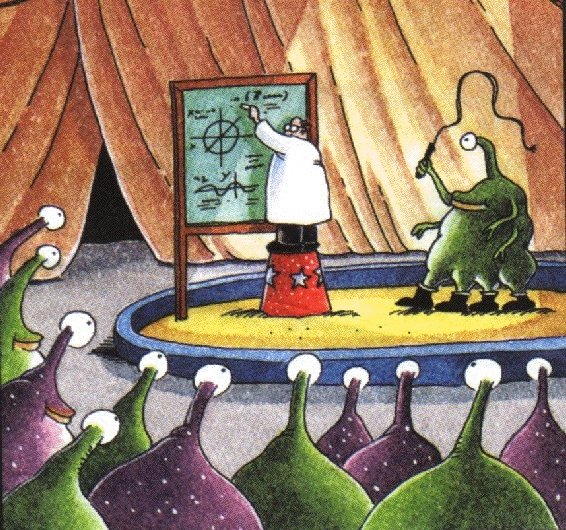
\includegraphics[height=4.5cm]{images/EventCalculus}
\end{center}
}



%\section{Outline}
\frame{
  \frametitle{Outline}
 \tableofcontents



}

\section{Welcome to MA211}

\frame{

This is Semester 1 of the Second Year Calculus course.

The basic information for the course is as follows:

\Bf{Lecturer:} \textbf{Dr Niall Madden, Dep of Mathematics}. My office is in
Room 103,
\href{http://www.maths.nuigalway.ie/~niall/NUIGalwayMapRiverside.jpg}{Riverside
  Terrapin}, Distillery Road.\\ 
Email:
\texttt{\href{mailto:Niall.Madden@NUIGalway.ie}{Niall.Madden@NUIGalway.ie}},
Phone (091 49) 3803.


\begin{center}
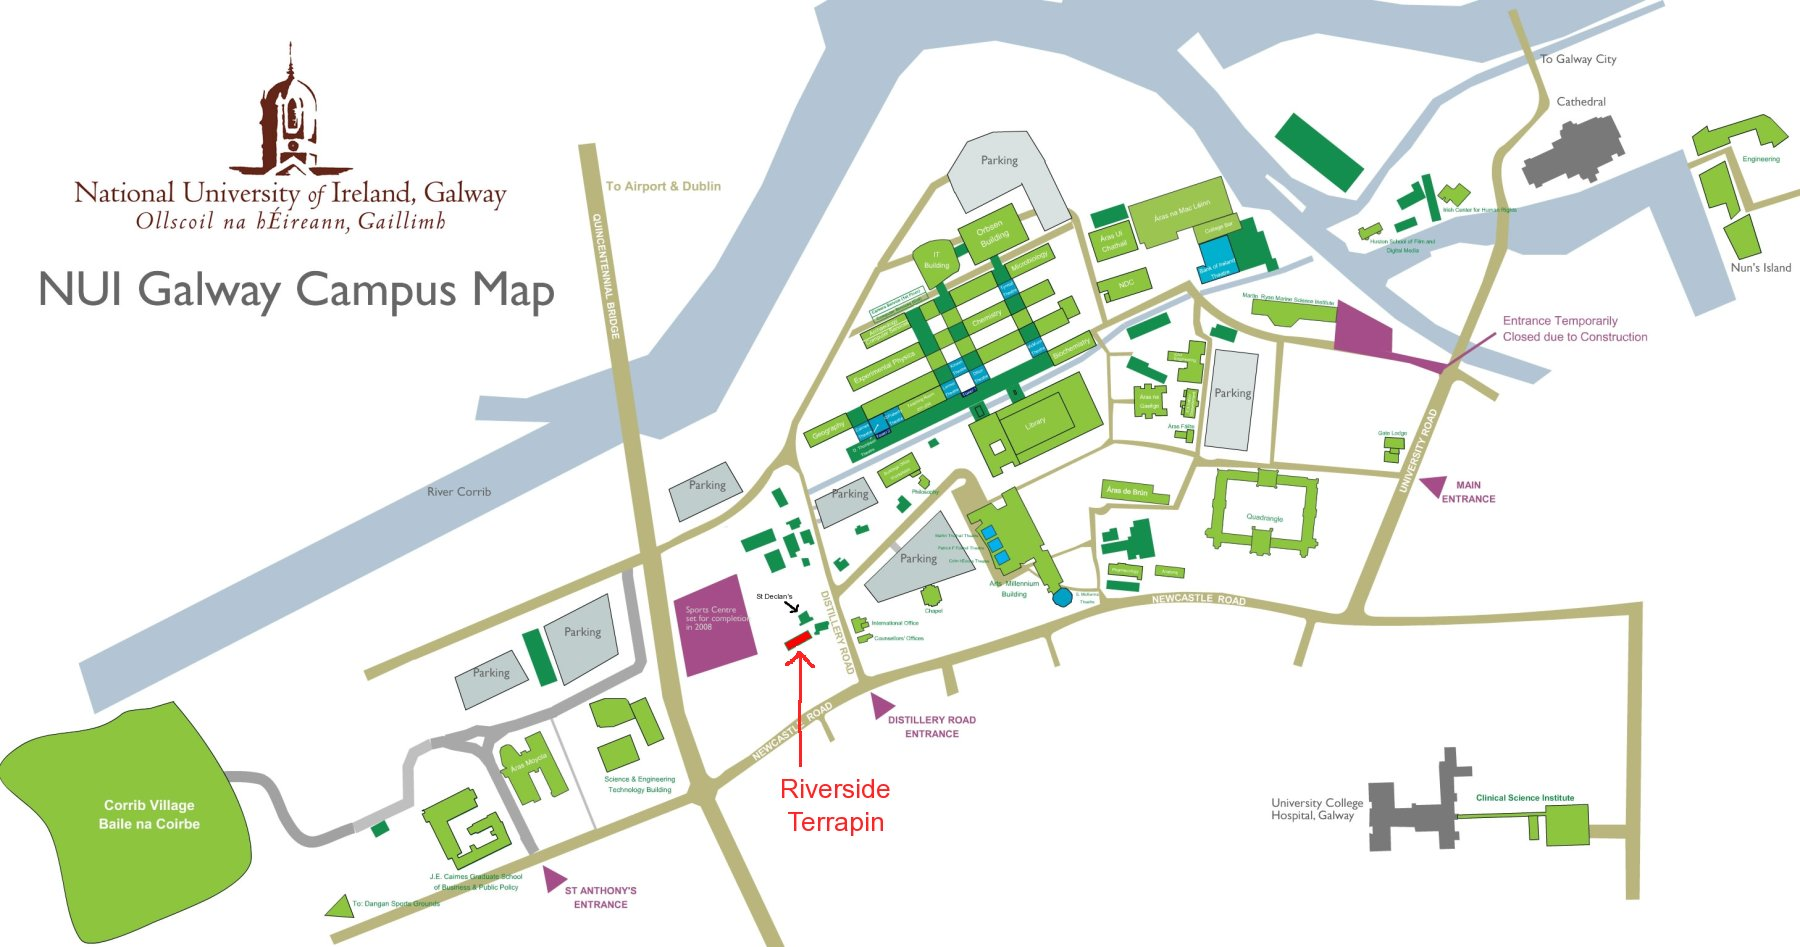
\includegraphics[width=9cm]{NUIGalwayMapRiverside}
\end{center}

}

\frame{
\begin{description}[<+->]
\item[Lectures:] Monday and Wednesday at 11 in the Cairnes Lecture Theatre.

\item[Tutorials:] \alert{To be arranged}. They will start during Week
  3, and  will deal with problem solving.



\item[Web site:] The on-line resources for this course are on
\href{http://BlackBoard.NUIGalway.ie}{\code{http://BlackBoard.NUIGalway.ie}}.
There you'll find various pieces of information, including these
notes.

It may take a week or two for everyone to have access to BlackBoard. 
In the short term, we'll also use
\href{http://www.maths.NUIGalway.ie/MA211}{\code{http://www.maths.NUIGalway.ie/MA211}}.




\end{description}
}

\section{Lecture Notes}

\frame{

\begin{center}

\includegraphics[width=2cm]{TakeNote}
\end{center}

A \Bf{summary of each lecture} will be posted to the site  no later
than 9.30 on the day of the lecture. 

\begin{center}
\Emph{Print these out and bring them with you to lectures.}
\end{center}

You will then annotate these notes during the class.

}

\section{Topics}

\frame{

The key topics in \Bf{MA211} are (but  not in order)
\begin{enumerate}[<+->]
\item Sets and functions.

\item  Methods of integration: substitution, integration by parts,
  partial fractions, reduction formulae. 

\item  Improper integrals (as limits of finite integrals).

\item Differential equations: linear equations with constant
  coefficients, first order homogeneous equations, boundary value
  problems, etc.

\end{enumerate}

}

\section{Mathematical Preliminaries}

\frame{

\begin{columns}[c]
\column{0.45\textwidth}

Anyone who can remember their first year calculus should be able for
this course.  

~

Where we make particular use of topics from 1st year, I will try to remind
you and give you a reference for a text-book.

~

If I don't, \alert{please ask!}

\column{0.55\textwidth}
\begin{center}
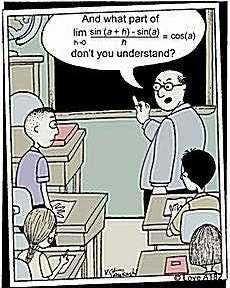
\includegraphics[width=5.5cm]{images/WhatPart}
\end{center}
\end{columns}


 
}

\section{Text book}
\frame{


There is no required textbook for this course, but two are
particularly recommended:
\begin{enumerate}[<+->]
\item Stewart: \Emph{Calculus} and \Emph{Calculus: early
    transcendentals}. Both are in the library. If buying a copy, get
  \Emph{Calculus}, rather than ``early transcendentals''.



\item Robert Adams, \Emph{Calculus: a short course, 3rd ED}, 515 ADA
%(Note: the library also has a few copies of the 5th ED. That one is
%less useful). 
There are 7 copies in the library.
\end{enumerate}

If you buy a copy of either of these, you will find it useful for MA211.

}
\frame{


Also useful are:

\begin{enumerate}
\item Anton, \Emph{Calculus}, 515 ANT


\item Spiegel, \Emph{Advanced Calculus}, 515 SPI (12 copies in the library)
-- This is only for the 1st half of the course.
\end{enumerate}

In general: any book with \Emph{Calculus} in the title and that covers 
\begin{itemize}[<+->]
\item Integration, including Improper Integrals
\item Transcendental functions, in particular exponential, logarithmic
  and hyperbolic functions.
\item Differential equations.
\end{itemize}

}


\section{Course assessment}
\frame{
Your progress in and commitment to this  course will be assessed as
follows:

\begin{itemize}
\item 
\Bf{Homework Assignment:}
There will be exercises included in every
  lecture. These will be collected into a series a problem sets which
  will be posted separately to Blackboard.  

  Every 3 weeks (approximately) you will be required to submit
  \Emph{carefully written solutions} to  selected exercises. These
  will be graded and returned to you. The mark you get will count
  towards you final MA211  grade 

\item 
\Bf{Class Test:}
 There will be a 30 minute class test during Week  6.

\item  \Bf{End of Semester Exam:}
Worth \Bf{75\%} of the total grade for
  MA211.
\end{itemize}

}




\section{What is Calculus?}

\frame{
 \textbf{Wikipedia:} 
\emph{Calculus (from Latin, "pebble" or "little stone") is a branch of mathematics that
  includes the study of limits, derivatives, integrals, and infinite
  series, and constitutes a major part of modern university
  education. 

Calculus has widespread applications in science and
  engineering and is used to solve complex and expansive problems for
  which algebra alone is insufficient. 

It builds on analytic geometry
  and mathematical analysis and includes two major branches,
  differential calculus and integral calculus, that are related by the
  fundamental theorem of calculus.
  }



}

\section{Exercises}

\frame{
\begin{enumerate}[<+->]


\item Goto to the library. Find where they keep the calculus
  books. Choose any three. Find the section where they introduce the
  concept of a \Bf{limit} of a function at a point. Write down the
  \Emph{definition of a limit} they provide, \Emph{their explanation
    of what it means}, and \emph{One example}.

Rank the books in order of how useful you think they are.

\item The study of what we call ``Calculus'' is said to have been
  started by \emph{Isaac Newton} and \emph{Gottfried  von
    Leibniz}.

Find out
  when and where they lived, and what their major mathematical
  discoveries were.

\end{enumerate}
} 



\end{document}

